% Auto-generated by generate_figures.py — do not edit manually
% Include in preamble: \usepackage{pgfplots}
\pgfplotsset{compat=1.18}
\usepackage{pgfplotstable}

% Include in body:     % Auto-generated by generate_figures.py — do not edit manually
% Include in preamble: \usepackage{pgfplots}
\pgfplotsset{compat=1.18}
\usepackage{pgfplotstable}

% Include in body:     % Auto-generated by generate_figures.py — do not edit manually
% Include in preamble: \usepackage{pgfplots}
\pgfplotsset{compat=1.18}
\usepackage{pgfplotstable}

% Include in body:     % Auto-generated by generate_figures.py — do not edit manually
% Include in preamble: \input{figures_preamble}
% Include in body:     \input{figures}


% ── Figure 1: Recall@1 vs Evidence Position ──────────────────────────────────
\begin{figure}[t]
\centering
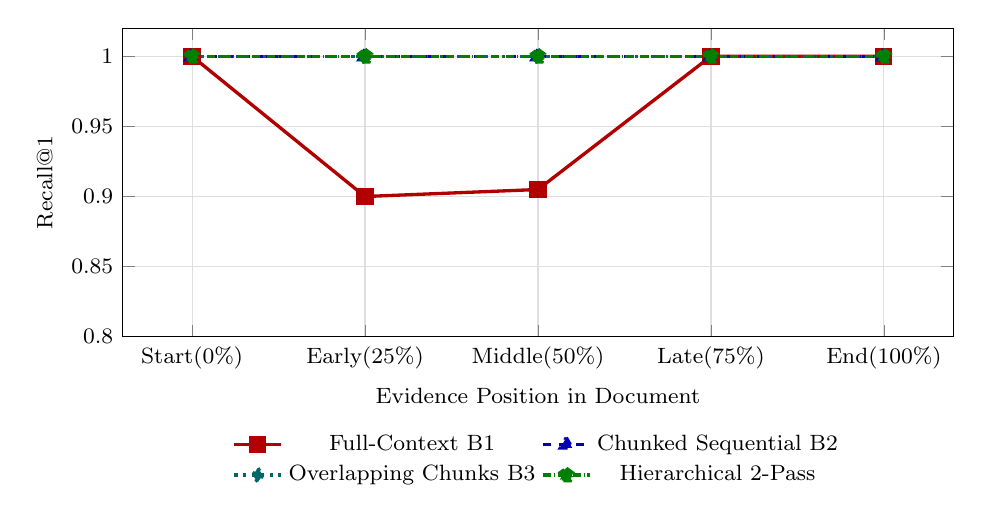
\begin{tikzpicture}
\begin{axis}[
  width=\columnwidth, height=5.5cm,
  xlabel={Evidence Position in Document},
  ylabel={Recall@1},
  ymin=0.80, ymax=1.02,
  xtick={1,2,3,4,5},
  xticklabels={Start\\(0\%),Early\\(25\%),Middle\\(50\%),Late\\(75\%),End\\(100\%)},
  legend style={at={(0.5,-0.28)}, anchor=north, legend columns=2,
                font=\footnotesize, draw=none},
  grid=major, grid style={gray!25},
  tick label style={font=\footnotesize},
  label style={font=\footnotesize},
  ymajorgrids=true,
  cycle list name=color list,
]
\addplot[color=red!70!black, mark=square*, solid, line width=1.2pt,
  mark size=2.5pt] coordinates {(1,1.0) (2,0.9) (3,0.905) (4,1.0) (5,1.0)};
\addlegendentry{Full-Context B1}
\addplot[color=blue!70!black, mark=triangle*, dashed, line width=1.2pt,
  mark size=2.5pt] coordinates {(1,1.0) (2,1.0) (3,1.0) (4,1.0) (5,1.0)};
\addlegendentry{Chunked Sequential B2}
\addplot[color=teal!80!black, mark=diamond*, dotted, line width=1.2pt,
  mark size=2.5pt] coordinates {(1,1.0) (2,1.0) (3,1.0) (4,1.0) (5,1.0)};
\addlegendentry{Overlapping Chunks B3}
\addplot[color=green!50!black, mark=pentagon*, densely dashdotted, line width=1.2pt,
  mark size=2.5pt] coordinates {(1,1.0) (2,1.0) (3,1.0) (4,1.0) (5,1.0)};
\addlegendentry{Hierarchical 2-Pass}
\end{axis}
\end{tikzpicture}
\caption{Recall@1 vs.\ evidence position for all four retrieval methods
  ($N=200$ trials per cell, random seed~42). The full-context baseline (FC-B1)
  drops to 0.900--0.905 at Early and Middle positions; all chunking methods
  maintain perfect recall across all positions.}
\label{fig:main}
\end{figure}


% ── Figure 2: Ablation — attention-decay strength ────────────────────────────
\begin{figure}[t]
\centering
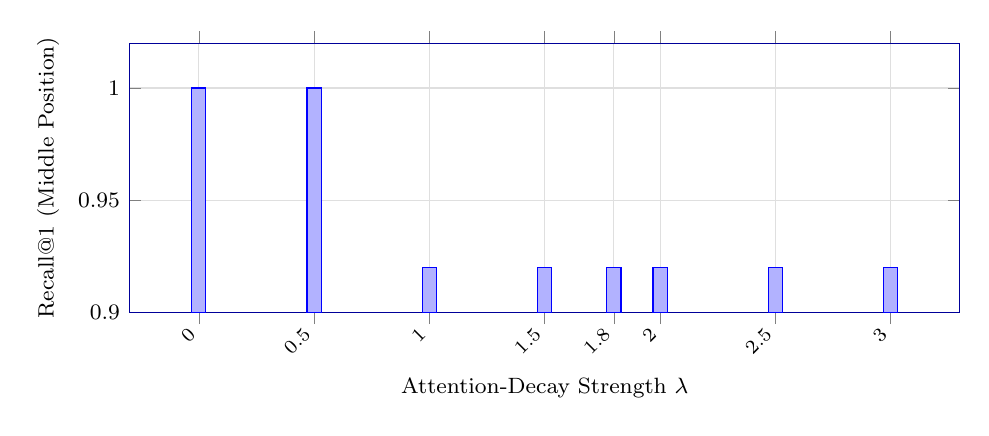
\begin{tikzpicture}
\begin{axis}[
  width=\columnwidth, height=5cm,
  xlabel={Attention-Decay Strength $\lambda$},
  ylabel={Recall@1 (Middle Position)},
  ymin=0.90, ymax=1.02,
  xtick={0,0.5,1,1.5,1.8,2,2.5,3},
  xticklabel style={font=\scriptsize, rotate=45, anchor=east},
  grid=major, grid style={gray!25},
  tick label style={font=\footnotesize},
  label style={font=\footnotesize},
  ybar, bar width=0.18cm,
  fill=blue!40, draw=blue!60!black,
]
\addplot coordinates {(0.0,1.0) (0.5,1.0) (1.0,0.92) (1.5,0.92) (1.8,0.92) (2.0,0.92) (2.5,0.92) (3.0,0.92)};

\end{axis}
\end{tikzpicture}
\caption{Ablation: Recall@1 of the Full-Context baseline at the Middle~(50\%)
  position as a function of attention-decay strength $\lambda$
  (Equation~\ref{eq:attn}, $N=200$ trials).
  Degradation is negligible below $\lambda=1.0$ and plateaus at 0.920 for
  all $\lambda \geq 1.0$, confirming robustness of the main result.}
\label{fig:ablation}
\end{figure}


% ── Figure 3: Average Recall across positions ────────────────────────────────
\begin{figure}[t]
\centering
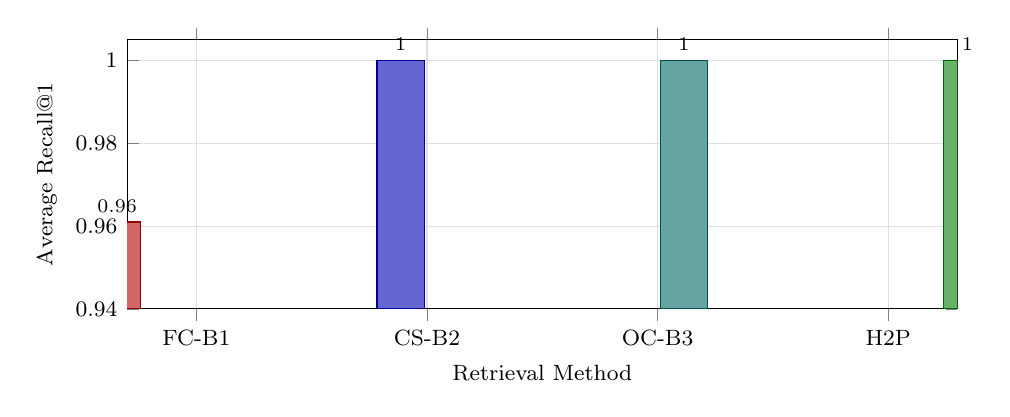
\begin{tikzpicture}
\begin{axis}[
  width=\columnwidth, height=5cm,
  xlabel={Retrieval Method},
  ylabel={Average Recall@1},
  ymin=0.94, ymax=1.005,
  xtick={1,2,3,4},
  xticklabels={FC-B1, CS-B2, OC-B3, H2P},
  grid=major, grid style={gray!25},
  tick label style={font=\footnotesize},
  label style={font=\footnotesize},
  nodes near coords, nodes near coords style={font=\scriptsize},
  ybar, bar width=0.6cm,
]
\addplot[fill=red!70!black!60, draw=red!70!black!80!black] coordinates {(1,0.9610)};
\addplot[fill=blue!70!black!60, draw=blue!70!black!80!black] coordinates {(2,1.0000)};
\addplot[fill=teal!80!black!60, draw=teal!80!black!80!black] coordinates {(3,1.0000)};
\addplot[fill=green!50!black!60, draw=green!50!black!80!black] coordinates {(4,1.0000)};
\end{axis}
\end{tikzpicture}
\caption{Average Recall@1 across all five evidence positions per method.
  FC-B1 scores 0.961 due to degradation at non-boundary positions;
  all three chunking methods achieve a perfect average of 1.000.}
\label{fig:avgrecall}
\end{figure}



% ── Figure 1: Recall@1 vs Evidence Position ──────────────────────────────────
\begin{figure}[t]
\centering
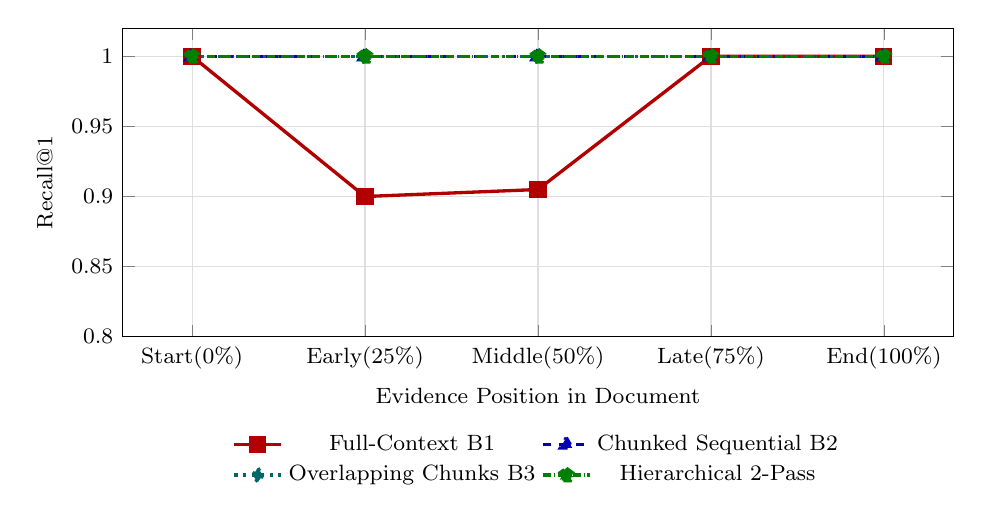
\begin{tikzpicture}
\begin{axis}[
  width=\columnwidth, height=5.5cm,
  xlabel={Evidence Position in Document},
  ylabel={Recall@1},
  ymin=0.80, ymax=1.02,
  xtick={1,2,3,4,5},
  xticklabels={Start\\(0\%),Early\\(25\%),Middle\\(50\%),Late\\(75\%),End\\(100\%)},
  legend style={at={(0.5,-0.28)}, anchor=north, legend columns=2,
                font=\footnotesize, draw=none},
  grid=major, grid style={gray!25},
  tick label style={font=\footnotesize},
  label style={font=\footnotesize},
  ymajorgrids=true,
  cycle list name=color list,
]
\addplot[color=red!70!black, mark=square*, solid, line width=1.2pt,
  mark size=2.5pt] coordinates {(1,1.0) (2,0.9) (3,0.905) (4,1.0) (5,1.0)};
\addlegendentry{Full-Context B1}
\addplot[color=blue!70!black, mark=triangle*, dashed, line width=1.2pt,
  mark size=2.5pt] coordinates {(1,1.0) (2,1.0) (3,1.0) (4,1.0) (5,1.0)};
\addlegendentry{Chunked Sequential B2}
\addplot[color=teal!80!black, mark=diamond*, dotted, line width=1.2pt,
  mark size=2.5pt] coordinates {(1,1.0) (2,1.0) (3,1.0) (4,1.0) (5,1.0)};
\addlegendentry{Overlapping Chunks B3}
\addplot[color=green!50!black, mark=pentagon*, densely dashdotted, line width=1.2pt,
  mark size=2.5pt] coordinates {(1,1.0) (2,1.0) (3,1.0) (4,1.0) (5,1.0)};
\addlegendentry{Hierarchical 2-Pass}
\end{axis}
\end{tikzpicture}
\caption{Recall@1 vs.\ evidence position for all four retrieval methods
  ($N=200$ trials per cell, random seed~42). The full-context baseline (FC-B1)
  drops to 0.900--0.905 at Early and Middle positions; all chunking methods
  maintain perfect recall across all positions.}
\label{fig:main}
\end{figure}


% ── Figure 2: Ablation — attention-decay strength ────────────────────────────
\begin{figure}[t]
\centering
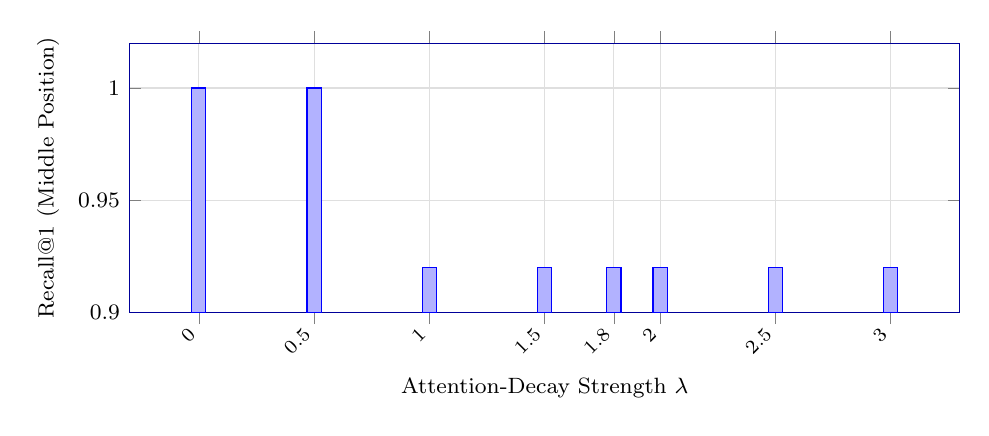
\begin{tikzpicture}
\begin{axis}[
  width=\columnwidth, height=5cm,
  xlabel={Attention-Decay Strength $\lambda$},
  ylabel={Recall@1 (Middle Position)},
  ymin=0.90, ymax=1.02,
  xtick={0,0.5,1,1.5,1.8,2,2.5,3},
  xticklabel style={font=\scriptsize, rotate=45, anchor=east},
  grid=major, grid style={gray!25},
  tick label style={font=\footnotesize},
  label style={font=\footnotesize},
  ybar, bar width=0.18cm,
  fill=blue!40, draw=blue!60!black,
]
\addplot coordinates {(0.0,1.0) (0.5,1.0) (1.0,0.92) (1.5,0.92) (1.8,0.92) (2.0,0.92) (2.5,0.92) (3.0,0.92)};

\end{axis}
\end{tikzpicture}
\caption{Ablation: Recall@1 of the Full-Context baseline at the Middle~(50\%)
  position as a function of attention-decay strength $\lambda$
  (Equation~\ref{eq:attn}, $N=200$ trials).
  Degradation is negligible below $\lambda=1.0$ and plateaus at 0.920 for
  all $\lambda \geq 1.0$, confirming robustness of the main result.}
\label{fig:ablation}
\end{figure}


% ── Figure 3: Average Recall across positions ────────────────────────────────
\begin{figure}[t]
\centering
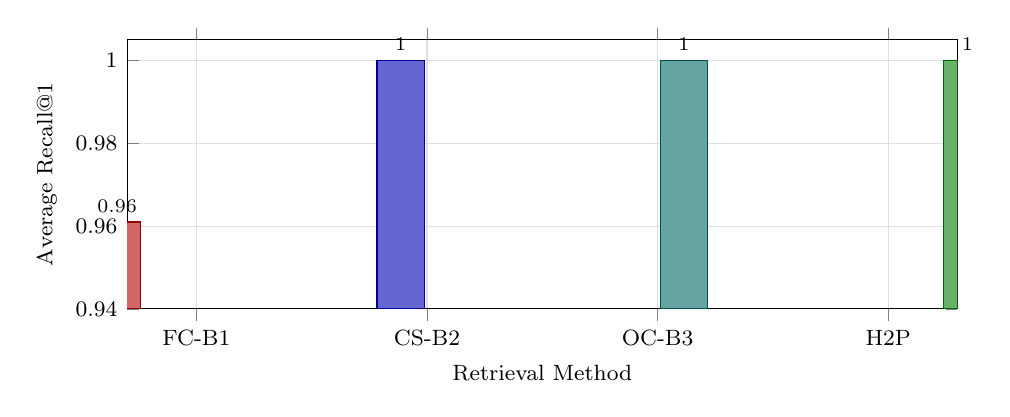
\begin{tikzpicture}
\begin{axis}[
  width=\columnwidth, height=5cm,
  xlabel={Retrieval Method},
  ylabel={Average Recall@1},
  ymin=0.94, ymax=1.005,
  xtick={1,2,3,4},
  xticklabels={FC-B1, CS-B2, OC-B3, H2P},
  grid=major, grid style={gray!25},
  tick label style={font=\footnotesize},
  label style={font=\footnotesize},
  nodes near coords, nodes near coords style={font=\scriptsize},
  ybar, bar width=0.6cm,
]
\addplot[fill=red!70!black!60, draw=red!70!black!80!black] coordinates {(1,0.9610)};
\addplot[fill=blue!70!black!60, draw=blue!70!black!80!black] coordinates {(2,1.0000)};
\addplot[fill=teal!80!black!60, draw=teal!80!black!80!black] coordinates {(3,1.0000)};
\addplot[fill=green!50!black!60, draw=green!50!black!80!black] coordinates {(4,1.0000)};
\end{axis}
\end{tikzpicture}
\caption{Average Recall@1 across all five evidence positions per method.
  FC-B1 scores 0.961 due to degradation at non-boundary positions;
  all three chunking methods achieve a perfect average of 1.000.}
\label{fig:avgrecall}
\end{figure}



% ── Figure 1: Recall@1 vs Evidence Position ──────────────────────────────────
\begin{figure}[t]
\centering
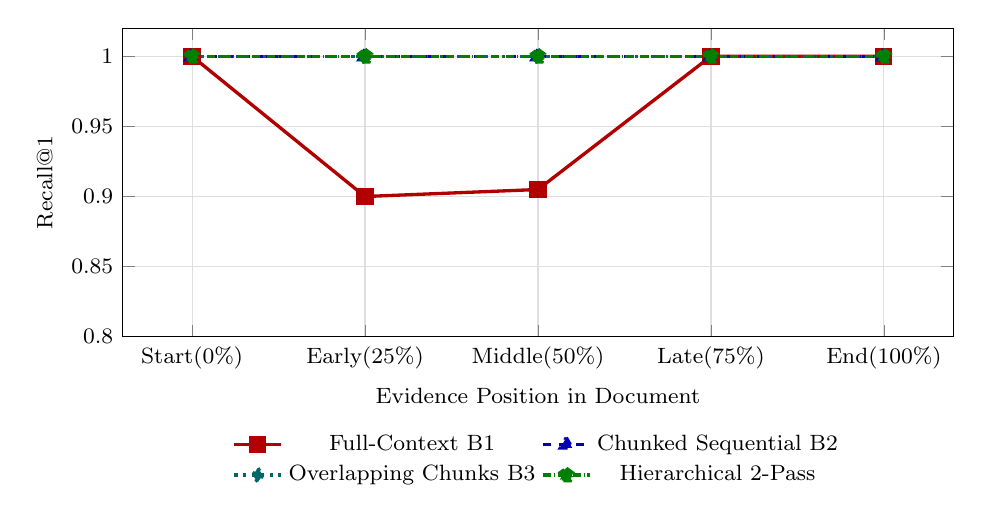
\begin{tikzpicture}
\begin{axis}[
  width=\columnwidth, height=5.5cm,
  xlabel={Evidence Position in Document},
  ylabel={Recall@1},
  ymin=0.80, ymax=1.02,
  xtick={1,2,3,4,5},
  xticklabels={Start\\(0\%),Early\\(25\%),Middle\\(50\%),Late\\(75\%),End\\(100\%)},
  legend style={at={(0.5,-0.28)}, anchor=north, legend columns=2,
                font=\footnotesize, draw=none},
  grid=major, grid style={gray!25},
  tick label style={font=\footnotesize},
  label style={font=\footnotesize},
  ymajorgrids=true,
  cycle list name=color list,
]
\addplot[color=red!70!black, mark=square*, solid, line width=1.2pt,
  mark size=2.5pt] coordinates {(1,1.0) (2,0.9) (3,0.905) (4,1.0) (5,1.0)};
\addlegendentry{Full-Context B1}
\addplot[color=blue!70!black, mark=triangle*, dashed, line width=1.2pt,
  mark size=2.5pt] coordinates {(1,1.0) (2,1.0) (3,1.0) (4,1.0) (5,1.0)};
\addlegendentry{Chunked Sequential B2}
\addplot[color=teal!80!black, mark=diamond*, dotted, line width=1.2pt,
  mark size=2.5pt] coordinates {(1,1.0) (2,1.0) (3,1.0) (4,1.0) (5,1.0)};
\addlegendentry{Overlapping Chunks B3}
\addplot[color=green!50!black, mark=pentagon*, densely dashdotted, line width=1.2pt,
  mark size=2.5pt] coordinates {(1,1.0) (2,1.0) (3,1.0) (4,1.0) (5,1.0)};
\addlegendentry{Hierarchical 2-Pass}
\end{axis}
\end{tikzpicture}
\caption{Recall@1 vs.\ evidence position for all four retrieval methods
  ($N=200$ trials per cell, random seed~42). The full-context baseline (FC-B1)
  drops to 0.900--0.905 at Early and Middle positions; all chunking methods
  maintain perfect recall across all positions.}
\label{fig:main}
\end{figure}


% ── Figure 2: Ablation — attention-decay strength ────────────────────────────
\begin{figure}[t]
\centering
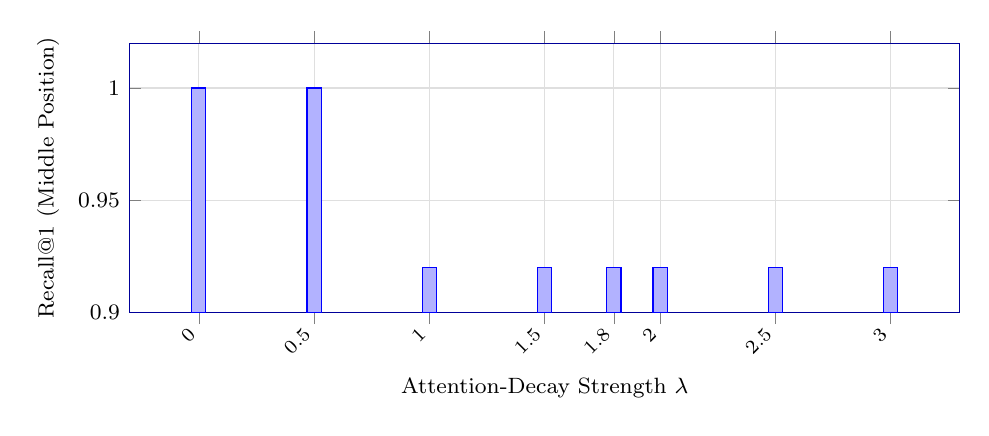
\begin{tikzpicture}
\begin{axis}[
  width=\columnwidth, height=5cm,
  xlabel={Attention-Decay Strength $\lambda$},
  ylabel={Recall@1 (Middle Position)},
  ymin=0.90, ymax=1.02,
  xtick={0,0.5,1,1.5,1.8,2,2.5,3},
  xticklabel style={font=\scriptsize, rotate=45, anchor=east},
  grid=major, grid style={gray!25},
  tick label style={font=\footnotesize},
  label style={font=\footnotesize},
  ybar, bar width=0.18cm,
  fill=blue!40, draw=blue!60!black,
]
\addplot coordinates {(0.0,1.0) (0.5,1.0) (1.0,0.92) (1.5,0.92) (1.8,0.92) (2.0,0.92) (2.5,0.92) (3.0,0.92)};

\end{axis}
\end{tikzpicture}
\caption{Ablation: Recall@1 of the Full-Context baseline at the Middle~(50\%)
  position as a function of attention-decay strength $\lambda$
  (Equation~\ref{eq:attn}, $N=200$ trials).
  Degradation is negligible below $\lambda=1.0$ and plateaus at 0.920 for
  all $\lambda \geq 1.0$, confirming robustness of the main result.}
\label{fig:ablation}
\end{figure}


% ── Figure 3: Average Recall across positions ────────────────────────────────
\begin{figure}[t]
\centering
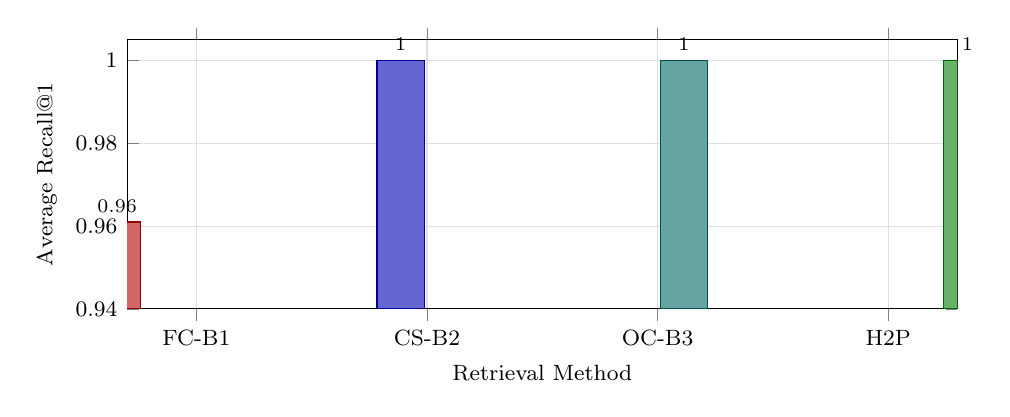
\begin{tikzpicture}
\begin{axis}[
  width=\columnwidth, height=5cm,
  xlabel={Retrieval Method},
  ylabel={Average Recall@1},
  ymin=0.94, ymax=1.005,
  xtick={1,2,3,4},
  xticklabels={FC-B1, CS-B2, OC-B3, H2P},
  grid=major, grid style={gray!25},
  tick label style={font=\footnotesize},
  label style={font=\footnotesize},
  nodes near coords, nodes near coords style={font=\scriptsize},
  ybar, bar width=0.6cm,
]
\addplot[fill=red!70!black!60, draw=red!70!black!80!black] coordinates {(1,0.9610)};
\addplot[fill=blue!70!black!60, draw=blue!70!black!80!black] coordinates {(2,1.0000)};
\addplot[fill=teal!80!black!60, draw=teal!80!black!80!black] coordinates {(3,1.0000)};
\addplot[fill=green!50!black!60, draw=green!50!black!80!black] coordinates {(4,1.0000)};
\end{axis}
\end{tikzpicture}
\caption{Average Recall@1 across all five evidence positions per method.
  FC-B1 scores 0.961 due to degradation at non-boundary positions;
  all three chunking methods achieve a perfect average of 1.000.}
\label{fig:avgrecall}
\end{figure}



% ── Figure 1: Recall@1 vs Evidence Position ──────────────────────────────────
\begin{figure}[t]
\centering
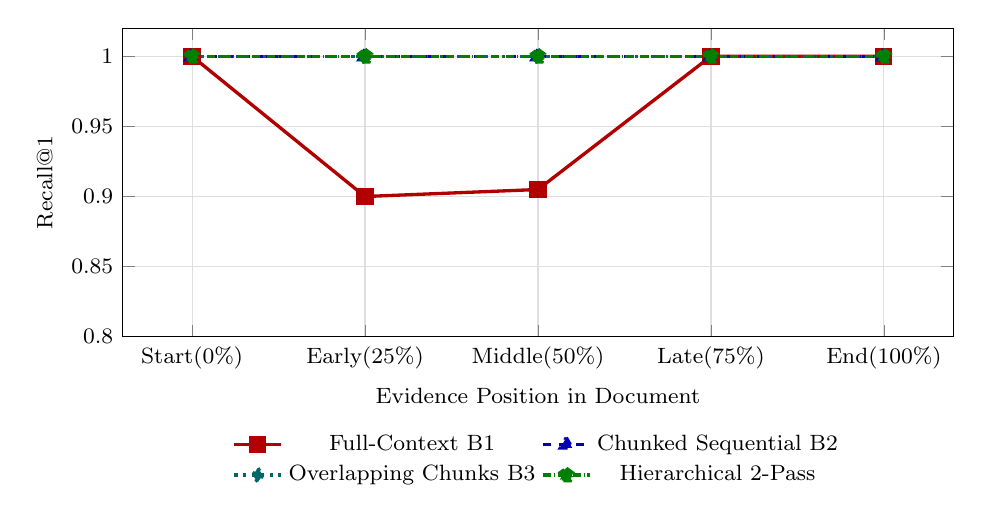
\begin{tikzpicture}
\begin{axis}[
  width=\columnwidth, height=5.5cm,
  xlabel={Evidence Position in Document},
  ylabel={Recall@1},
  ymin=0.80, ymax=1.02,
  xtick={1,2,3,4,5},
  xticklabels={Start\\(0\%),Early\\(25\%),Middle\\(50\%),Late\\(75\%),End\\(100\%)},
  legend style={at={(0.5,-0.28)}, anchor=north, legend columns=2,
                font=\footnotesize, draw=none},
  grid=major, grid style={gray!25},
  tick label style={font=\footnotesize},
  label style={font=\footnotesize},
  ymajorgrids=true,
  cycle list name=color list,
]
\addplot[color=red!70!black, mark=square*, solid, line width=1.2pt,
  mark size=2.5pt] coordinates {(1,1.0) (2,0.9) (3,0.905) (4,1.0) (5,1.0)};
\addlegendentry{Full-Context B1}
\addplot[color=blue!70!black, mark=triangle*, dashed, line width=1.2pt,
  mark size=2.5pt] coordinates {(1,1.0) (2,1.0) (3,1.0) (4,1.0) (5,1.0)};
\addlegendentry{Chunked Sequential B2}
\addplot[color=teal!80!black, mark=diamond*, dotted, line width=1.2pt,
  mark size=2.5pt] coordinates {(1,1.0) (2,1.0) (3,1.0) (4,1.0) (5,1.0)};
\addlegendentry{Overlapping Chunks B3}
\addplot[color=green!50!black, mark=pentagon*, densely dashdotted, line width=1.2pt,
  mark size=2.5pt] coordinates {(1,1.0) (2,1.0) (3,1.0) (4,1.0) (5,1.0)};
\addlegendentry{Hierarchical 2-Pass}
\end{axis}
\end{tikzpicture}
\caption{Recall@1 vs.\ evidence position for all four retrieval methods
  ($N=200$ trials per cell, random seed~42). The full-context baseline (FC-B1)
  drops to 0.900--0.905 at Early and Middle positions; all chunking methods
  maintain perfect recall across all positions.}
\label{fig:main}
\end{figure}


% ── Figure 2: Ablation — attention-decay strength ────────────────────────────
\begin{figure}[t]
\centering
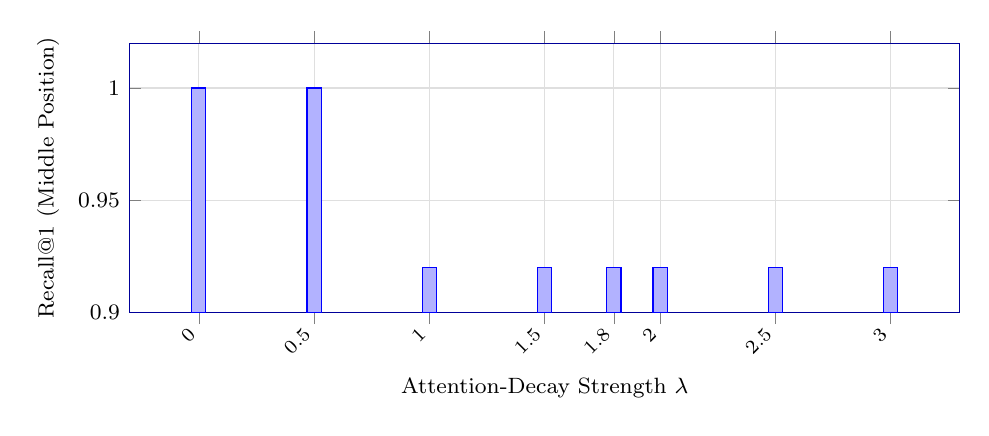
\begin{tikzpicture}
\begin{axis}[
  width=\columnwidth, height=5cm,
  xlabel={Attention-Decay Strength $\lambda$},
  ylabel={Recall@1 (Middle Position)},
  ymin=0.90, ymax=1.02,
  xtick={0,0.5,1,1.5,1.8,2,2.5,3},
  xticklabel style={font=\scriptsize, rotate=45, anchor=east},
  grid=major, grid style={gray!25},
  tick label style={font=\footnotesize},
  label style={font=\footnotesize},
  ybar, bar width=0.18cm,
  fill=blue!40, draw=blue!60!black,
]
\addplot coordinates {(0.0,1.0) (0.5,1.0) (1.0,0.92) (1.5,0.92) (1.8,0.92) (2.0,0.92) (2.5,0.92) (3.0,0.92)};

\end{axis}
\end{tikzpicture}
\caption{Ablation: Recall@1 of the Full-Context baseline at the Middle~(50\%)
  position as a function of attention-decay strength $\lambda$
  (Equation~\ref{eq:attn}, $N=200$ trials).
  Degradation is negligible below $\lambda=1.0$ and plateaus at 0.920 for
  all $\lambda \geq 1.0$, confirming robustness of the main result.}
\label{fig:ablation}
\end{figure}


% ── Figure 3: Average Recall across positions ────────────────────────────────
\begin{figure}[t]
\centering
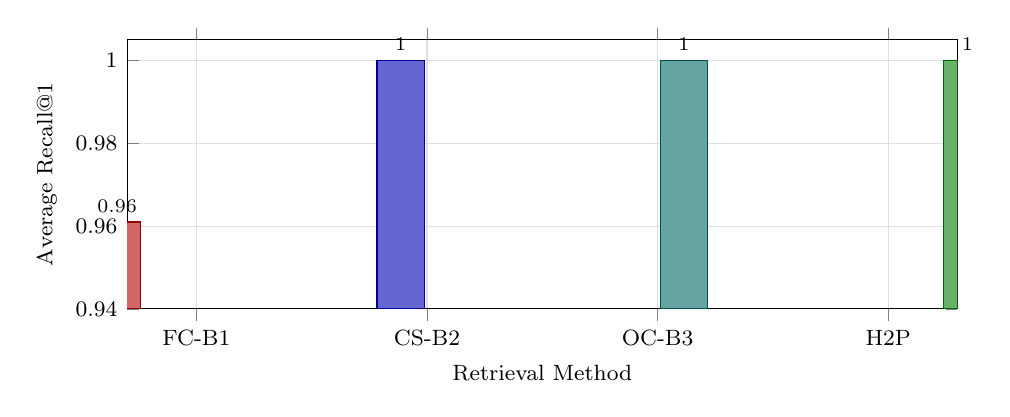
\begin{tikzpicture}
\begin{axis}[
  width=\columnwidth, height=5cm,
  xlabel={Retrieval Method},
  ylabel={Average Recall@1},
  ymin=0.94, ymax=1.005,
  xtick={1,2,3,4},
  xticklabels={FC-B1, CS-B2, OC-B3, H2P},
  grid=major, grid style={gray!25},
  tick label style={font=\footnotesize},
  label style={font=\footnotesize},
  nodes near coords, nodes near coords style={font=\scriptsize},
  ybar, bar width=0.6cm,
]
\addplot[fill=red!70!black!60, draw=red!70!black!80!black] coordinates {(1,0.9610)};
\addplot[fill=blue!70!black!60, draw=blue!70!black!80!black] coordinates {(2,1.0000)};
\addplot[fill=teal!80!black!60, draw=teal!80!black!80!black] coordinates {(3,1.0000)};
\addplot[fill=green!50!black!60, draw=green!50!black!80!black] coordinates {(4,1.0000)};
\end{axis}
\end{tikzpicture}
\caption{Average Recall@1 across all five evidence positions per method.
  FC-B1 scores 0.961 due to degradation at non-boundary positions;
  all three chunking methods achieve a perfect average of 1.000.}
\label{fig:avgrecall}
\end{figure}
